\addchapheadtotoc
\chapter{Context and related works}
 In this chapter, we introduce graph networks, how they arise from real world problems. Then we present the graph classification problem and the applications in which it can be used. After that, we proceed to state-of-the-art methods and its limitations, and we finish be stating our contribution. 
\section{Graph structures and its presence in real world}
Formally, a graph of size $v$ is a pair $\mathcal{G}=(\mathcal{V},\mathcal{E})$, where $\mathcal{V}=\{u_1,...,u_v\}$ is a set of  graph nodes, and $\mathcal{E}\in \mathcal{V}\times \mathcal{V}$ is the set of edges between these nodes, i.e. $(u_i, u_j)\in \mathcal{E}$ means that the graph has an edge between node $u_i$ and node $u_j$.
Graph structures are used to represent a set of objects and the interactions/relations that link between different pairs of these objects.  While the nature of these objects and their interactions vary depending on the application, they are still represented the same way where objects are reduced to nodes, and a relation between two objects is reduced to an edge between the corresponding two nodes. For example, Fig. \ref{fig:Graph_Example} shows how we can represent chemical reactions mechanisms by  graph structures.\newline
The need to graph structures and its analysis can be traced back to 1679, when G.W.  Leibniz  wrote to C. Huygens about the limitations of traditional analysis methods of geometric figures and said that "we need yet another kind of analysis, geometric or linear, which deals directly with position, as algebra deals with magnitude", \citep{Graph_application}. Then it was the invent of graph structures, which provided a pictorial form to represent data instead of using a lot of words to do so. With graph structures, these data become easier to be processed and analyzed, and that helps solving many problems that have been unsolved before \citep{Graph_application}.
\begin{figure}[H]
\centering
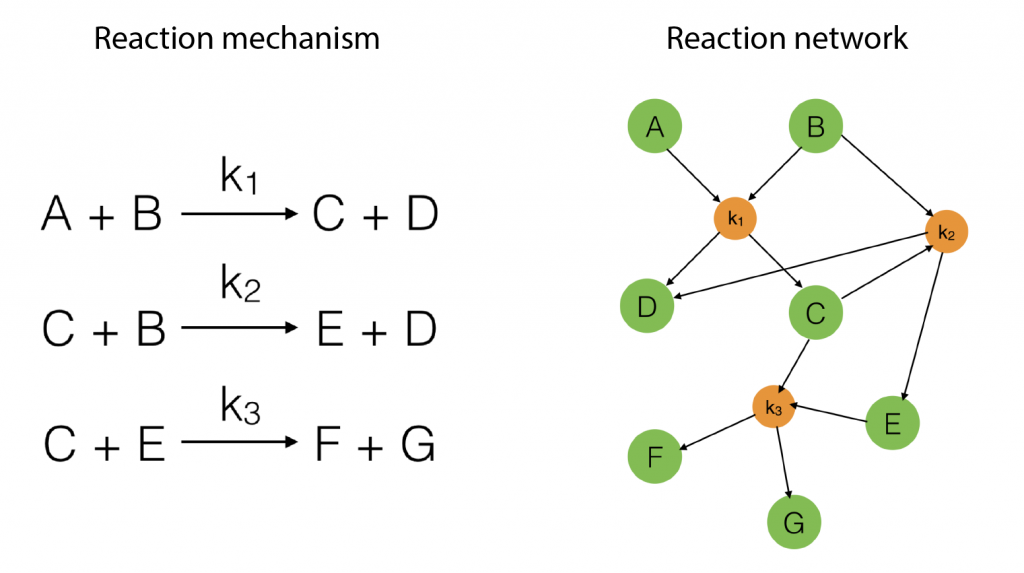
\includegraphics[scale=0.2]{figs/Graph_example.png}
\caption[Graph example to represent Chemical Reactions]{Graph structures in representing chemical reactions mechanisms}
%Source:
\label{fig:Graph_Example}
\end{figure}
To better understand how graphs are built in real life, we show in Table.\ref{table:Graph_examples} some examples of these graphs in different domains.

\begin{table}
\small
\begin{center}
\begin{tabular}{|c|c|c|c|c|}
\hline
{Network}  &  {Nodes} & {Node features}  & {Edges}  & {Edge features}  \\
\hline
{Transportation System}  &  {cities} & {registered cars}  & {Routes}  & {Length, cost }  \\
\hline
{Banking Network}  &  {Account holders} & {account status}  & {Transactions}  & {Transaction value}  \\
\hline
{Social Network}  &  {users} & {name, country}  & {Interactions}  & {type (like, comment)}  \\
\hline
\end{tabular}
\end{center}
\caption{Some real world graphs}
\label{table:Graph_examples}
\end{table}

\section{Graph classification problem}
\label{sec:Graph_classification_problem}
Let's consider the case when we have a set $\mathcal{D}$ of all valid graphs $\mathcal{G}$ that can occur in some real-world domain, a fixed set of classes/categories $\beta=\{\beta _1,\ldots,\beta _l\}$ of finite size $l$, and a mapping function $f:\mathcal{D}\mapsto\beta$ which maps each graph $\mathcal{G}$ in $\mathcal{D}$ to the class $\beta_\mathcal{G}$ it belongs to. Graph classification is the problem of estimating the mapping function $f$ in the case where it is only known on a subset $\mathcal{X}\subset \mathcal{D}$. Formally, we have a dataset $(\mathcal{X}=\{\mathcal{G}_1,\ldots,\mathcal{G}_n\}, \mathcal{Y}=\{y_1,\ldots,y_n\})$ of size $n$ such that $\mathcal{X}\in \mathcal{D}^n$ and $\mathcal{Y}\in\beta^n$, where for each graph $\mathcal{G}_i\in \mathcal{X}$ we have that $y_i=f(\mathcal{G}_i)$ is the class of $\mathcal{G}_i$, and that is why it is called labeled dataset. The classification task is to have a \textbf{predictive model} which can predict well, based on some-predefined metric,  the class for any new graph $\mathcal{G}$ in $\mathcal{D}$ not only in $\mathcal{X}$. This prediction functionality of the model is gained using the dataset $(\mathcal{X}, \mathcal{Y})$ to optimize the parameters of the model that is believed to govern the behavior of the mapping function $f$ on $\mathcal{D}$. This optimization completed in this paradigm is called the learning algorithm.\newline
In some applications each node/edge in the graph dataset has its own features vector that can be used along with the graph structure to classify different graphs into different classes, while in other applications all we have is the graph structure or it happens that some nodes/edges have their features but others don't. In this project, we consider the one case of graph classification with the absence of any node/edge features.
In practice, this problem is drastically being addressed in many fields, as in:
\begin{itemize}
    \item \textbf{\emph{Marketing analytics:}} advertisers and marketers  are interested in detecting the influential people communities in Social Networks in the sense that addressing their products' advertisements to such groups would be a more rewarding investment. This can be approached with graph classification applied on these networks \citep{marketing_analytics}.
    \item \textbf{\emph{Banking security:}} graph classification is used to catch unusual patterns of fraudulent transactions \citep{banking_security}.
    \item \textbf{\emph{Biology and genomics:}} graphs are based on proteins such that nodes correspond
to amino acids which compound the protein and a pair of amino acids are linked by an edge if they are less than 6 Angstroms apart. The task is to detect whether a protein is an enzyme or not \citep{protein_application}, to mention a few.
\end{itemize}

\section{State-of-the-art methods for graph classification}
We  present here the traditional algorithms deployed in graph classification problem, we simultaneously state the limitations of each of them. In general, these algorithms can be traced back into four main categories: Set based, frequent sub-graph based, kernel based, and graph neural networks based algorithms.\newline 
\textbf{\emph{Set based algorithms:}} this type of algorithms is particularly applied on graphs whose nodes/edges are supplied with features or attributes, so each graph is reduced to  a set of nodes, edges or both. Then a distance function of interest between the graphs is computed  based on the similarity between pairs of edges/nodes in the corresponding sets. The drawback of this method is that it does not take the structure (topology) of the graph itself into consideration. For example, if we just compare how much the edges of one graph are similar to the ones of another, we can have two graphs with the same set of edge features, which will lead to maximum similarity, but we in reality ignore other important information that can make these graphs completely different such that how many connected communities of nodes these edges form in each graph, how many circles of nodes these edges promote in each graph, etc. On the other hand, a strength point of these algorithms  compared to others is the low computations cost that is usually linear or quadratic in the number of nodes and edges \citep{graphlet_kernel}.\newline 
\textbf{\emph{Frequent sub-graph based algorithms:}} these algorithms can be applied in two stages, the graph dataset (all the graphs we have  in an application) is first analyzed to pick the frequent sub-graphs that occur in different graphs. Then, another analysis is done to choose the most discriminative sub-graphs out of the ones resulted from the first stage. The disadvantage of using this method is the computational cost that grows exponentially with the graph size \citep{graphlet_kernel}. \newline
\textbf{\emph{Graph kernels based algorithms:}} it is a middle ground between both previous methodologies, where the graph structure (topology) is well considered, and in most cases, these algorithms are designed in a way that the computational time is a polynomial function of the graph size \citep{graphlet_kernel}. However, some effective and competitive kernels still require exponential time, and this is in short the problem we approached in this work using random features to approximate these kernels or to compete them in notably lower computational time. \newline
\textbf{\emph{Graph neural networks (GNNs) based algorithms:}} GNNs revolutionized learning on graph structures, as it computes a representation vector (embedding vector) for every node in the graph, where this vector is recursively computed by aggregating the representation vectors of neighbor nodes. The goal of this aggregation technique is that nodes that are neighbors (or even close) to each other in the graph are more likely to have a similar representations (with respect to some similarity function) and vise versa. On the graph level, a representation vector is computed by aggregating its nodes representation vectors, and then this vector is used as the features vector which can be fed to a typical deep neural network to learn the classification task. Traditional GNNs such as graph convolutional networks (GCNs) and GraphSAGE failed to provide high performance classifying graphs whose node/edges don't include any original features vectors,  and that even applies on graphs with simple topology \citep{GCN_powerful}. 
However, another GNN structure was developed to overcome this weakness point, and it is referred to by Graph Isomorphism Network (GIN). Regarding the computational time, it is mainly a matter of the layers number in the network, since this parameter in reality represents how far from a node we want to go in order to compute its representation vector. 

\section{Context and our contribution}
$K$-graphlet kernel is one of the aforementioned graph kernels which has proven to be  competitive in graph classification. Theoretically and empirically, it was shown that a desired performance or a required amount of information to be preserved from the original graph can be reached with sufficiently large $k$. However,  the computational cost  ecomes prohibitive as ($k$: the graphlet size) and/or ($v$: the size of the graph to be sampled)  become too large. Thus it cannot be applied on large-scale graph datasets. The advent of Optical Processing Units (OPUs) opened a new horizon solving this problem, since it can apply enormous number of \emph{Random Projections} in light speed. \newline
In this work, we did the sufficient mathematical analysis to prove that OPUs' light-speed random feature projections compete the $k$-graphlet kernel with respect to \emph{Maximum Mean Discrepancy (MMD)} Euclidean metric. Moreover, we empirically tested this hypothesis and made sure that the the theoretical MMD error is aligned with the empirical one with respect to the parameters introduced in the problem (sampling technique, number of sampled sub-graphs, number of random features, etc). 





